\fancyhead[LO,LE]{}
\fancyhead[RO,RE]{\textsf{\textbf{MỤC 1.4}}\quad \textsf{Hàm số mũ}\quad \textbf{49}}

\noindent
\begin{minipage}[t]{0.26\textwidth}
    \vspace{0pt}
    \centering
    {\small \textbf{\textsf{BẢNG 1}}\quad \textsf{Dân số thế giới}}
    \vspace{4pt}
    
    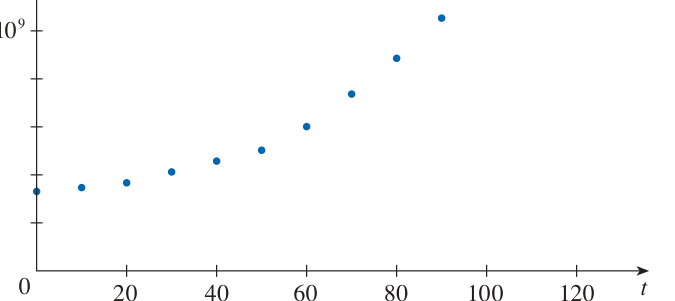
\includegraphics[width=\linewidth]{images/p0084_fig1.png}
\end{minipage}%
\hfill
\begin{minipage}[t]{0.71\textwidth}
    \vspace{0pt}
    Từ quy luật này, có vẻ như trong trường hợp tổng quát, ta có
    \[
    p(t) = 2^t \times 1000 = (1000)2^t
    \]
    Hàm dân số này là một bội số hằng của hàm số mũ $y = 2^t$, do đó nó thể hiện sự tăng trưởng nhanh chóng mà chúng ta đã quan sát trong Hình~7. Dưới các điều kiện lý tưởng (không gian và dinh dưỡng không giới hạn, không có dịch bệnh), sự tăng trưởng theo hàm mũ này là điển hình cho những gì thực sự xảy ra trong tự nhiên.
    \par\vspace{0.66em}
    \noindent
    \textbf{\textsf{\color{stewartcyan}VÍ DỤ 3}}\quad Bảng 1 cho thấy dữ liệu về dân số thế giới trong thế kỷ 20 và Hình~8 biểu diễn biểu đồ phân tán tương ứng.
    \par\vspace{0.41em}
    Quy luật của các điểm dữ liệu trong Hình~8 gợi ý sự tăng trưởng theo hàm mũ, vì vậy chúng ta sử dụng một máy tính bỏ túi có chức năng vẽ đồ thị (hoặc máy tính điện tử) có khả năng hồi quy hàm mũ để áp dụng phương pháp bình phương bé nhất và thu được mô hình hàm mũ
    \[
    P(t) = (1{,}43653 \times 10^9) \cdot (1{,}01395)^t
    \]
    trong đó $t = 0$ tương ứng với năm 1900. Hình~9 cho thấy đồ thị của hàm số mũ này cùng với các điểm dữ liệu ban đầu. Ta thấy rằng đường cong hàm mũ khớp với dữ liệu khá tốt. Giai đoạn tăng trưởng dân số tương đối chậm được giải thích bởi hai cuộc chiến tranh thế giới và cuộc Đại suy thoái vào những năm 1930.
\end{minipage}

\vspace{0.98em}
\noindent
\begin{minipage}[t]{0.48\textwidth}
    \centering
    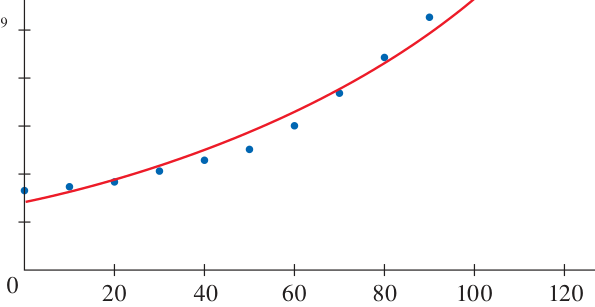
\includegraphics[width=\linewidth]{images/p0084_fig2.png}
    \vspace{4pt}
    
    {\small \textbf{\textsf{HÌNH 8}}\quad \textsf{Biểu đồ phân tán cho sự tăng trưởng dân số thế giới}}
\end{minipage}%
\hfill
\begin{minipage}[t]{0.48\textwidth}
    \centering
    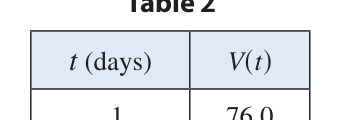
\includegraphics[width=\linewidth]{images/p0084_fig3.png}
    \vspace{4pt}
    
    {\small \textbf{\textsf{HÌNH 9}}\quad \textsf{Mô hình hàm mũ cho sự tăng trưởng dân số thế giới}\hfill{\color{stewartcyan}$\blacksquare$}}
\end{minipage}

\vspace{1.23em}
\noindent
\begin{minipage}[t]{0.26\textwidth}
    \vspace{0pt}
    \centering
    {\small \textbf{\textsf{BẢNG 2}}}
    \vspace{4pt}
    
    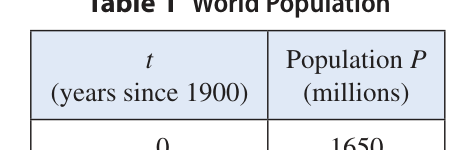
\includegraphics[width=\linewidth]{images/p0084_fig4.png}
\end{minipage}%
\hfill
\begin{minipage}[t]{0.71\textwidth}
    \vspace{0pt}
    \textbf{\textsf{\color{stewartcyan}VÍ DỤ 4}}\quad Vào năm 1995, một bài báo nghiên cứu đã được công bố trình bày chi tiết về tác dụng của chất ức chế protease ABT-538 đối với virus gây suy giảm miễn dịch ở người HIV-1.$^1$ Bảng 2 thể hiện các giá trị tải lượng virus trong huyết tương $V(t)$ của bệnh nhân 303, được đo bằng số lượng bản sao RNA trên mỗi mL, sau $t$ ngày kể từ khi bắt đầu điều trị bằng ABT-538. Biểu đồ phân tán tương ứng được thể hiện trong Hình~10 (ở trang tiếp theo).
    \par\vspace{0.41em}
    Sự suy giảm khá mạnh của tải lượng virus mà chúng ta thấy trong Hình~10 gợi nhớ đến đồ thị của hàm số mũ $y = b^x$ trong các Hình~3 và 4(a) đối với trường hợp cơ số $b$ nhỏ hơn 1. Vì vậy, chúng ta hãy mô hình hóa hàm số $V(t)$ bằng một hàm số mũ. Sử dụng máy tính cầm tay có chức năng đồ họa hoặc máy tính điện tử để khớp dữ liệu trong Bảng 2 với một hàm mũ

    \vspace{2.05em}
    \noindent\rule{0.45\textwidth}{0.4pt}\\[4pt]
    {\footnotesize 1. D. Ho và cộng sự, “Rapid Turnover of Plasma Virions and CD4 Lymphocytes in HIV-1 Infection,” \textit{Nature} 373 (1995): 123--26.}
\end{minipage}